\documentclass{standalone}
\usepackage{tikz}
\usetikzlibrary{patterns, positioning}


\begin{document}
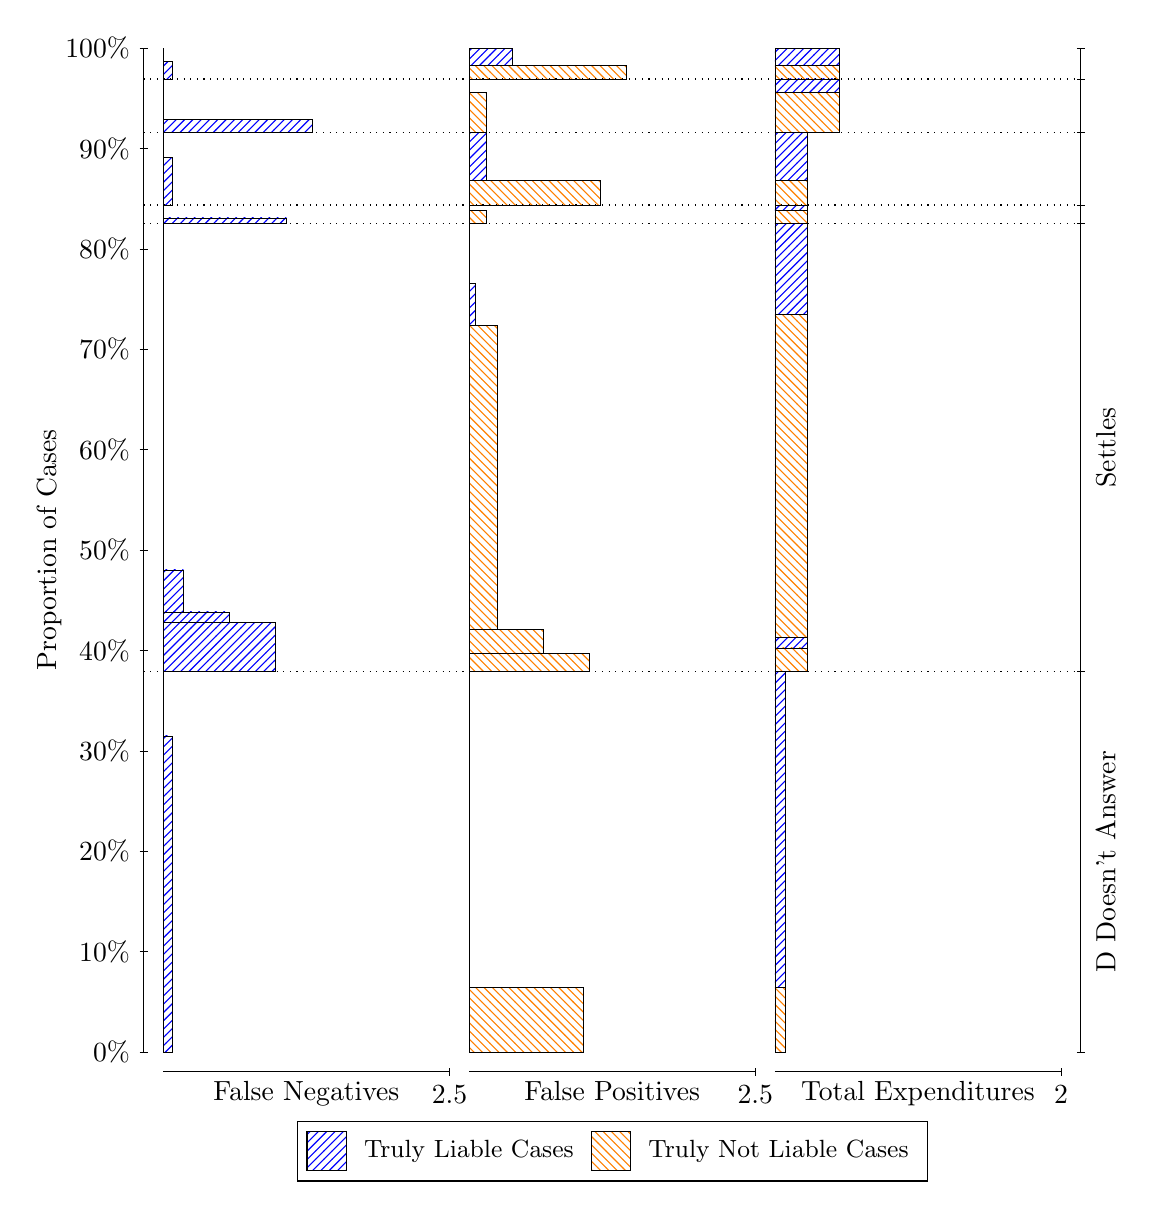
\begin{tikzpicture}
\draw[black, very thin] (1.5,1.75) -- (1.5,14.5);
\node[rotate=90, text=black, anchor=center] at (0.3, 8.125) {Proportion of Cases};
\draw[black, very thin] (1.45,1.75) -- (1.55,1.75);
\node[text=black, anchor=east] at (1.45, 1.75) {0\%};
\draw[black, very thin] (1.45,3.025) -- (1.55,3.025);
\node[text=black, anchor=east] at (1.45, 3.025) {10\%};
\draw[black, very thin] (1.45,4.3) -- (1.55,4.3);
\node[text=black, anchor=east] at (1.45, 4.3) {20\%};
\draw[black, very thin] (1.45,5.575) -- (1.55,5.575);
\node[text=black, anchor=east] at (1.45, 5.575) {30\%};
\draw[black, very thin] (1.45,6.85) -- (1.55,6.85);
\node[text=black, anchor=east] at (1.45, 6.85) {40\%};
\draw[black, very thin] (1.45,8.125) -- (1.55,8.125);
\node[text=black, anchor=east] at (1.45, 8.125) {50\%};
\draw[black, very thin] (1.45,9.4) -- (1.55,9.4);
\node[text=black, anchor=east] at (1.45, 9.4) {60\%};
\draw[black, very thin] (1.45,10.675) -- (1.55,10.675);
\node[text=black, anchor=east] at (1.45, 10.675) {70\%};
\draw[black, very thin] (1.45,11.95) -- (1.55,11.95);
\node[text=black, anchor=east] at (1.45, 11.95) {80\%};
\draw[black, very thin] (1.45,13.225) -- (1.55,13.225);
\node[text=black, anchor=east] at (1.45, 13.225) {90\%};
\draw[black, very thin] (1.45,14.5) -- (1.55,14.5);
\node[text=black, anchor=east] at (1.45, 14.5) {100\%};

\draw[black, very thin] (13.4,1.75) -- (13.4,14.5);
\draw[black, very thin] (13.35,1.75) -- (13.45,1.75);
\node[anchor=west] at (13.35, 1.75) {};
\draw[black, very thin] (13.35,6.5808) -- (13.45,6.5808);
\node[anchor=west] at (13.35, 6.5808) {};
\draw[black, very thin] (13.35,12.271) -- (13.45,12.271);
\node[anchor=west] at (13.35, 12.271) {};
\draw[black, very thin] (13.35,12.506) -- (13.45,12.506);
\node[anchor=west] at (13.35, 12.506) {};
\draw[black, very thin] (13.35,13.424) -- (13.45,13.424);
\node[anchor=west] at (13.35, 13.424) {};
\draw[black, very thin] (13.35,14.107) -- (13.45,14.107);
\node[anchor=west] at (13.35, 14.107) {};
\draw[black, very thin] (13.35,14.5) -- (13.45,14.5);
\node[anchor=west] at (13.35, 14.5) {};

\draw[black, very thin, pattern color=blue, pattern=north east lines] (1.75,1.75) rectangle (1.859,5.7639);
\draw[black, very thin, pattern color=orange, pattern=north west lines] (1.75,5.7639) rectangle (1.75,6.5808);
\draw[black, very thin, pattern color=blue, pattern=north east lines] (1.75,6.5808) rectangle (3.167,7.2036);
\draw[black, very thin, pattern color=blue, pattern=north east lines] (1.75,7.2036) rectangle (2.5857,7.3378);
\draw[black, very thin, pattern color=blue, pattern=north east lines] (1.75,7.3378) rectangle (2.0043,7.8731);
\draw[black, very thin, pattern color=orange, pattern=north west lines] (1.75,7.8731) rectangle (1.75,12.271);
\draw[black, very thin, pattern color=blue, pattern=north east lines] (1.75,12.271) rectangle (3.3123,12.343);
\draw[black, very thin, pattern color=orange, pattern=north west lines] (1.75,12.343) rectangle (1.75,12.506);
\draw[black, very thin, pattern color=blue, pattern=north east lines] (1.75,12.506) rectangle (1.859,13.109);
\draw[black, very thin, pattern color=orange, pattern=north west lines] (1.75,13.109) rectangle (1.75,13.424);
\draw[black, very thin, pattern color=blue, pattern=north east lines] (1.75,13.424) rectangle (3.6393,13.595);
\draw[black, very thin, pattern color=orange, pattern=north west lines] (1.75,13.595) rectangle (1.75,14.107);
\draw[black, very thin, pattern color=blue, pattern=north east lines] (1.75,14.107) rectangle (1.859,14.33);
\draw[black, very thin, pattern color=orange, pattern=north west lines] (1.75,14.33) rectangle (1.75,14.5);
\draw[black, very thin, pattern color=orange, pattern=north west lines] (5.6333,1.75) rectangle (7.0867,2.5669);
\draw[black, very thin, pattern color=blue, pattern=north east lines] (5.6333,2.5669) rectangle (5.6333,6.5808);
\draw[black, very thin, pattern color=orange, pattern=north west lines] (5.6333,6.5808) rectangle (7.1593,6.8137);
\draw[black, very thin, pattern color=orange, pattern=north west lines] (5.6333,6.8137) rectangle (6.578,7.1159);
\draw[black, very thin, pattern color=orange, pattern=north west lines] (5.6333,7.1159) rectangle (5.9967,10.979);
\draw[black, very thin, pattern color=blue, pattern=north east lines] (5.6333,10.979) rectangle (5.706,11.514);
\draw[black, very thin, pattern color=blue, pattern=north east lines] (5.6333,11.514) rectangle (5.6333,12.271);
\draw[black, very thin, pattern color=orange, pattern=north west lines] (5.6333,12.271) rectangle (5.8513,12.435);
\draw[black, very thin, pattern color=blue, pattern=north east lines] (5.6333,12.435) rectangle (5.6333,12.506);
\draw[black, very thin, pattern color=orange, pattern=north west lines] (5.6333,12.506) rectangle (7.3047,12.821);
\draw[black, very thin, pattern color=blue, pattern=north east lines] (5.6333,12.821) rectangle (5.8513,13.424);
\draw[black, very thin, pattern color=orange, pattern=north west lines] (5.6333,13.424) rectangle (5.8513,13.936);
\draw[black, very thin, pattern color=blue, pattern=north east lines] (5.6333,13.936) rectangle (5.6333,14.107);
\draw[black, very thin, pattern color=orange, pattern=north west lines] (5.6333,14.107) rectangle (7.6317,14.277);
\draw[black, very thin, pattern color=blue, pattern=north east lines] (5.6333,14.277) rectangle (6.1783,14.5);
\draw[black, very thin, pattern color=orange, pattern=north west lines] (9.5167,1.75) rectangle (9.6529,2.5669);
\draw[black, very thin, pattern color=blue, pattern=north east lines] (9.5167,2.5669) rectangle (9.6529,6.5808);
\draw[black, very thin, pattern color=orange, pattern=north west lines] (9.5167,6.5808) rectangle (9.9254,6.883);
\draw[black, very thin, pattern color=blue, pattern=north east lines] (9.5167,6.883) rectangle (9.9254,7.0172);
\draw[black, very thin, pattern color=orange, pattern=north west lines] (9.5167,7.0172) rectangle (9.9254,11.113);
\draw[black, very thin, pattern color=blue, pattern=north east lines] (9.5167,11.113) rectangle (9.9254,12.271);
\draw[black, very thin, pattern color=orange, pattern=north west lines] (9.5167,12.271) rectangle (9.9254,12.435);
\draw[black, very thin, pattern color=blue, pattern=north east lines] (9.5167,12.435) rectangle (9.9254,12.506);
\draw[black, very thin, pattern color=orange, pattern=north west lines] (9.5167,12.506) rectangle (9.9254,12.821);
\draw[black, very thin, pattern color=blue, pattern=north east lines] (9.5167,12.821) rectangle (9.9254,13.424);
\draw[black, very thin, pattern color=orange, pattern=north west lines] (9.5167,13.424) rectangle (10.334,13.936);
\draw[black, very thin, pattern color=blue, pattern=north east lines] (9.5167,13.936) rectangle (10.334,14.107);
\draw[black, very thin, pattern color=orange, pattern=north west lines] (9.5167,14.107) rectangle (10.334,14.277);
\draw[black, very thin, pattern color=blue, pattern=north east lines] (9.5167,14.277) rectangle (10.334,14.5);
\draw[black, dotted] (1.5,6.5808) -- (13.4,6.5808);
\draw[black, dotted] (1.5,12.271) -- (13.4,12.271);
\draw[black, dotted] (1.5,12.506) -- (13.4,12.506);
\draw[black, dotted] (1.5,13.424) -- (13.4,13.424);
\draw[black, dotted] (1.5,14.107) -- (13.4,14.107);
\draw[black, very thin] (1.75,1.5) -- (5.3833,1.5);
\node[text=black, anchor=north] at (3.5667, 1.5) {False Negatives};
\draw[black, very thin] (5.3833,1.45) -- (5.3833,1.55);
\node[text=black, anchor=north] at (5.3833, 1.45) {2.5};

\draw[black, very thin] (5.6333,1.5) -- (9.2667,1.5);
\node[text=black, anchor=north] at (7.45, 1.5) {False Positives};
\draw[black, very thin] (9.2667,1.45) -- (9.2667,1.55);
\node[text=black, anchor=north] at (9.2667, 1.45) {2.5};

\draw[black, very thin] (9.5167,1.5) -- (13.15,1.5);
\node[text=black, anchor=north] at (11.333, 1.5) {Total Expenditures};
\draw[black, very thin] (13.15,1.45) -- (13.15,1.55);
\node[text=black, anchor=north] at (13.15, 1.45) {2};

\node[text=black, centered, rotate=90] at (13.72, 4.1654) {D Doesn't Answer};
\node[text=black, centered, rotate=90] at (13.72, 9.4261) {Settles};





\draw (7.449999999999999,1.5) node[draw=none] (baseCoordinate) {};
\begin{scope}[align=center]
        \matrix[scale=0.5, draw=black, below=0.5cm of baseCoordinate, nodes={draw}, column sep=0.1cm]{
            \node[rectangle, draw, minimum width=0.5cm, minimum height=0.5cm, pattern color=blue, pattern=north east lines] {}; &
            \node[draw=none, font=\small, text=black] (B) {Truly Liable Cases}; &
            \node[rectangle, draw, minimum width=0.5cm, minimum height=0.5cm, pattern color=orange, pattern=north west lines] {}; &
            \node[draw=none, font=\small, text=black] (B) {Truly Not Liable Cases}; \\
            };
\end{scope}

\end{tikzpicture}
\end{document}